\index{KIWI images!workflow|(}
\chapter{Basic workflow}
\label{chapter:workflow}
\minitoc

The creation of an image with KIWI is always divided into two
basic steps. These are the \textbf{prepare} and the \textbf{create}
step. the create step requires the prepare step to be exited
successfully. Within this first prepare step kiwi builds of a new root
tree or, in kiwi-speak, a new physical extend. The building of a new
root tree consists of the creation of the directory specified to
hold it and the installation of the selected packages on it. The
installation of software packages is driven by a packagemanager.
KIWI supports the smart and zypper package managers. The prepare
step executes the following major stages:

\begin{itemize}
\item \textbf{Root directory creation}\\
      To prevent accidental deletion of an existing root tree, kiwi will
      stop with an error message if this folder already exists, unless the
      option --force-new-root is used in which case the existing root will
      be deleted.
\item \textbf{Package installation}\\
      First the selected package manager (smart by default) is instructed to
      use the repositories specified in the image description file.
      Then the packages specified in the 'bootstrap' section are installed.
      These packages are installed externally to the target root system
      (i.e. not chroot'ed) and establish the initial environment so the rest
      of  the process may run chroot'ed. Essential packages in this section
      are filesystem and glibc-locale. In practice you only need to
      specify those two, since the rest of the packages will be pulled
      because of the dependency system. To save space in your image you
      could schedule a set of packages for deletion after the package
      installation phase is over by listing them in the 'delete' section.
\item \textbf{User defined script config.sh}\\
      At the end of the preperation stage the optional script named config.sh
      is called. This script should be used to configure the system which means
      for example the activation of services. For a detailed description what
      functions are already available to configure the system please refer to
      the KIWI::config.sh manual page
\item \textbf{Managing the new root tree}\\
      At this point you can make changes on your physical extend so it fits
      your purpose better. Bear in mind that changes at this point will be
      discarded and not repeated automatically if you rerun the 'prepare'
      phase unless you include them in your original config.xml file and/or
      config.sh script. Please also note that the image description has
      been copied into the new root below the directory
      \textbf{<new-root>/image}. Any subsequent create step will read
      the image description information from the new root tree and not
      from the original image description location. According to this
      if you need to change the image description data
      after the prepare call has finished you need to change it inside the
      new root tree as well as in your original description directory to
      prevent loosing the change when your root tree will be removed later
      for some reason.
\end{itemize}

After the prepare step has finished successfully a subsequent building of
an image file or, in kiwi-speak, a new logical extend follows.
The building of an image requires a successfully prepared new root
tree in the first place. Using this tree multiple image types can be
created. So to speak it's possible to create a VMware image and a
XEN image from the same prepared root tree. The create step executes the
following major stages:

\begin{itemize}
\item \textbf{User defined script images.sh}\\
      At the beginning of the creation stage the optional script named
      images.sh is called. This script has no distinctive use case like
      config.sh but is most often used to remove packages which were pulled
      in by a dependency but are not really required for the later use
      of the operating system. For a detailed description what
      functions are already available to images.sh please refer to
      the KIWI::images.sh manual page
\item \textbf{Create the requested image type}\\
      What image type(s) a kiwi image supports depends on what types has been
      setup in the main image description file config.xml. At least one type
      must be setup. The following picture shows what image types are
      currently supported by kiwi:

      \begin{figure}[h]
      \centering
      \includegraphics[scale=0.5]{pictures/types.eps}
      \caption{Image Types}
      \label{fig:types}
      \end{figure}
\end{itemize}

Detailed information including a step by step guidance how to call
kiwi and how to make use of the result image can be found in the image
type specific sections later in this document.

\section{Boot process}
Todays linux systems are using a special boot image to control the
boot process. This boot image is called \textbf{initrd}. The linux
kernel loads this initial ramdisk which is a compressed cpio archive
into RAM and calls init or if present the program named linuxrc. The
KIWI image system also takes care for the creation of this boot image.
Each image type has it's own special boot code and shares the common
parts in a set of module functions. The image descriptions for the
boot images are provided by KIWI and thus the user has in almost all
cases no need to take care for the boot image.

\begin{figure}[h]
\centering
\includegraphics[scale=0.5]{pictures/activation.eps}
\caption{Boot process}
\label{fig:initrd}
\end{figure}

Furthermore KIWI automatically creates this boot image along with
the requested image type. It does that by calling itself in a prepare
and create call. There is no difference in terms of the description
of such a boot image compared to the system image description. The
system image description is the one the user creates and this image
represents the later operating system whereas the boot image only
lives temporarly in RAM as long as the system image will be activated.
The boot image descriptions are stores in /usr/share/kiwi/image/*boot
and can be build in the same way as the system image. The boot image
without a corresponding system image doesn't make sense though.

\section{Boot parameters}
When booting an image created by kiwi using one of the provided
boot images there are some useful kernel parameters mainly meant
for debugging purposes. Please note the following parameters are
only useful if the kiwi initrd is used. In case of any other
initrd code written by yourself or simply because kiwi replaced
itself with the distribution specfic mkinitrd tool the parameters
might not have any effect.

\begin{itemize}
\item \textbf{kiwidebug=1}\\
      If the boot process encounters a fatal error the system normally
      reacts with a reboot after 120 secconds. This so called exception
      can be influenced by the kiwidebug parameter. If set to 1 the system
      will stop and provide the user with a shell prompt instead of a
      reboot. Within that shell some basic standard commands are
      available which could help to find the cause of the problem
\item \textbf{kiwistderr=/dev/...}\\
      While the system boots kiwi writes messages to tty1 and tty3. The
      tty1 messages are highlevel information whereas the tty3 messages
      represents the shell debug output and any error messages from
      the commands called. With the kiwistderr parameter one can combine
      both message sets and specify where to write them to. It's very
      common to set /dev/console as possible alternative to the default
      logging behaviour
\end{itemize}

\section{Common and Distribution specific code}
KIWI has been developed to be usable for any Linux distribution.
By design of a Linux distribution there are differences between
each of them. With KIWI we provide on one hand the code which
is common to all Linux distributions according to standards and
on the other hand there is also code where we have to distinguish
between the distribution type.

In case of such specific tasks which are almost all in the area
of booting, KIWI provides a set of functions which all have to come
with a distribution prefix. As this project uses SUSE Linux as
base distribution all required distribution specific tasks has been
implemented for SUSE and could be missing for other distributions.
The existing implementation for SUSE turns out to be adapted to other
distributions very easily though.

A look into the code therefore will show you functions which are
prefixed by ''suse'' as well as scripts whose names starts with
''suse-''. At any time you see such a script or function
you can be assured that this is something distribution specific
and needs to be adapted if you plan to use KIWI with another
distribution than SUSE. For example the boot workflow is controlled
by a program called linuxrc which is in KIWI a script represented
by suse-linuxrc. Another example would be the function called
suseStripKernel which is able to remove everything but a specified
list of kernel drivers from the SUSE kernel.

The prefixed implementation allows us to integrate all the
distribution specific tasks into one project but this of course
requires the help and knowledge of the people who are familar
with their preferred linux distribution. 
